%!TEX root = batch-course.tex

\begin{frame}\frametitle{Batch PCA example: SBR}
	
	\begin{itemize}
		\item	Simulated data from \emph{large} mechanistic model for styrene butadiene rubber
		
		\item	Good to start learning from this case study
		
		\item	Simulated to contain ``normal operating conditions''
		
				\begin{itemize}
					\item	2 main problematic batches
					
					\item	same fault, but starting at different times
				\end{itemize}
	\end{itemize}
	
\end{frame}

\defverbatim[colored]\loaddata{%
\begin{lstlisting}[basicstyle=\tt\scriptsize,frame=none,language=C++,linewidth=.9\textwidth]

data = load('datasets/SBR.mat');   % X is in a  10600 x 9 matrix
Y_data = data.Y;
   
% Specify the data dimensions
nBatches = 53;
nTags = 6;
nSamples = 200;  % not required
tagNames = {'Reactor temperature', 'Cooling water temp', ...
            'Reactor jacket temperature', 'Latex density', ...
            'Conversion', 'Energy released'};
        
% Create a batch block first: tell it how many batches 
% there are in the aligned data
% Ignore tags 1, 2, 3 (noisy and uninformative)

batchX = block(data.X(:, 4:9), 'X', 'batch', ...
               'tagNames', tagNames, 'nBatches', nBatches);
\end{lstlisting}}

\begin{frame}[fragile,containsverbatim]\frametitle{SBR: load the data}
	\loaddata
\end{frame}

\begin{frame}\frametitle{SBR: raw data}
	
	\begin{itemize}
		\item	Batches: \( N = 53 \); Tags: \( K = 6 \); Time steps: \( J = 200 \)
		
	\end{itemize}
	
	\begin{center}
		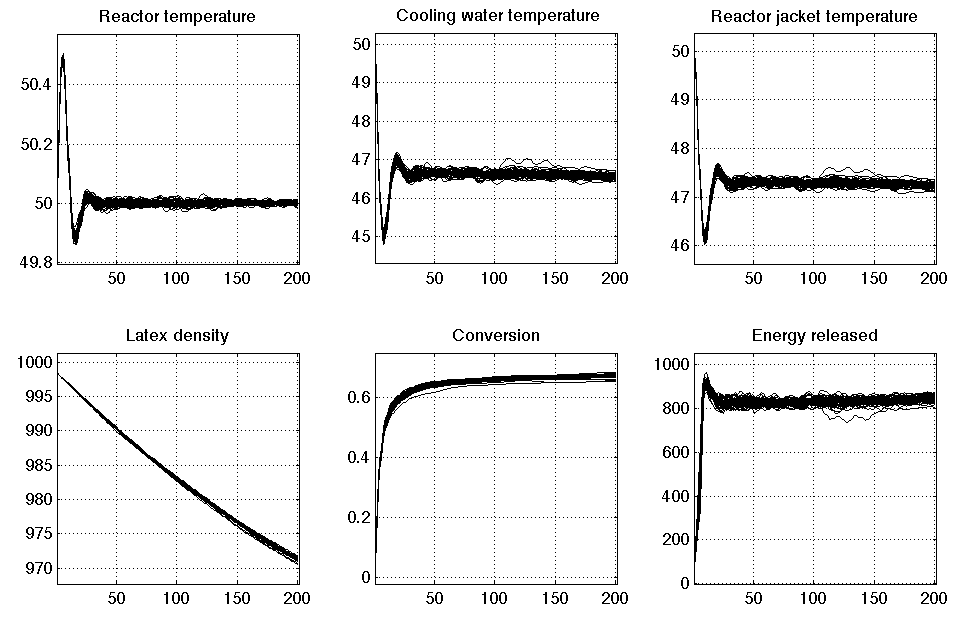
\includegraphics[width=\textwidth]{images/sbr/SBR-raw-data-trajectories.png}
	\end{center}
	{\color{myOrange}{\texttt{plot(batchX, 'raw', 2, 3)}}}
\end{frame}

\begin{frame}\frametitle{SBR: build model}
	
	\begin{itemize}
		\item	Start with 2 to 3 components: \emph{just to see what's going on}
		
		\item	{\color{myOrange}{\texttt{batch\_PCA = lvm(\{'X', batchX\}, 2)}}}
		
		\item	\( R^2_1 = 24.5\% \) and \( R^2_2 = 13.3\% \)
		
		\item	Next: scores, loadings, SPE, \( T^2 \): all the usual PCA tools
		
	\end{itemize}

\end{frame}

\begin{frame}\frametitle{SBR: scores and \( T^2 \)}
	
	\begin{center}
		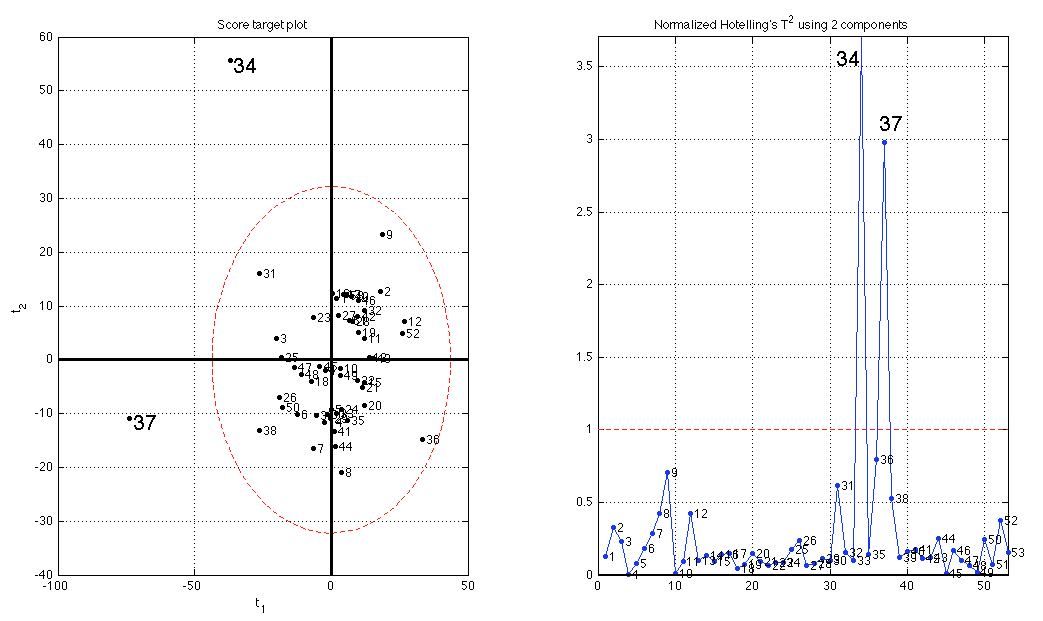
\includegraphics[width=0.8\textwidth]{images/sbr/SBR-scores-and-T2.png}
	\end{center}

	\begin{itemize}
		\item	{\color{myOrange}{\texttt{plot(batch\_PCA, 'scores')}}}
		
		\item	Batch 34 and 37 had differences from bulk of data in their progress.\pause
		
		\item	These were in fact the unsuccessful batches!  This shows promise.
	\end{itemize}

\end{frame}

\begin{frame}\frametitle{SBR: check SPE}
	
	\begin{center}
		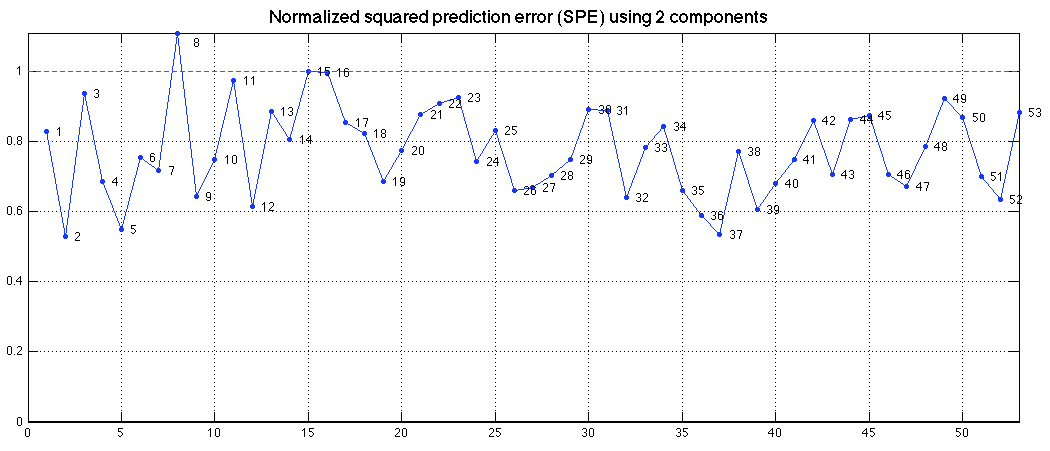
\includegraphics[width=0.8\textwidth]{images/sbr/SBR-SPE-plot-per-batch.png}
	\end{center}

	\begin{itemize}
		\item	{\color{myOrange}{\texttt{plot(batch\_PCA, 'spe')}}}
		
		\item	No problems picked up.  This is the overall SPE, for the \emph{entire} batch.
	\end{itemize}

\end{frame}

\begin{frame}\frametitle{SBR: understand \( R^2 \) breakdown}
	
	\begin{center}
		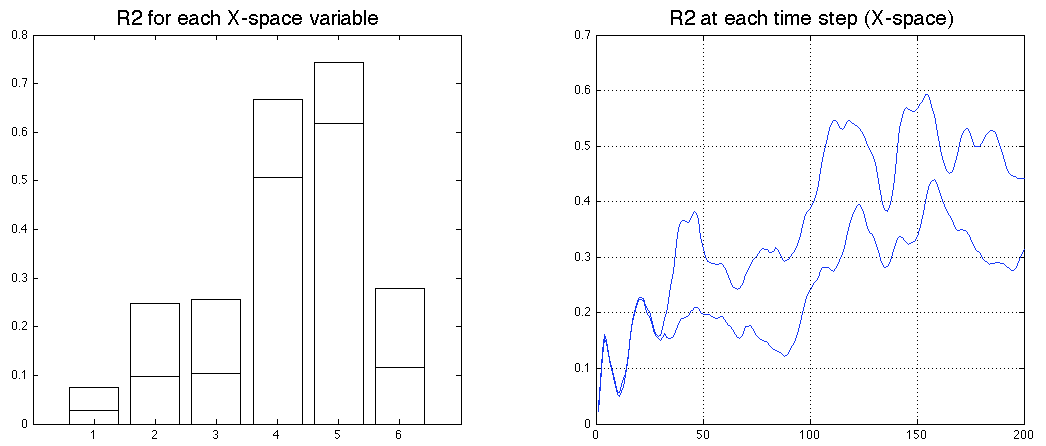
\includegraphics[width=0.8\textwidth]{images/sbr/SBR-R2-over-batch.png}
	\end{center}

	\begin{itemize}
		\item	{\color{myOrange}{\texttt{plot(batch\_PCA, 'R2')}}}
		
		\item	LV1: Tags 4 (latex density) and 5 (conversion) dominate
		
		\item	LV2: explains tags 2, 3, 4, 5, 6 by about 15\% each
		
		\item	LV1: explains everything over \( t = 0 \)  to \( t = 30 \)
		
		\item	\( R^2 \) is low at start because all batches are similar initially
		
				\begin{itemize}
					\item	after centering and scaling there is just noise at the start.
				\end{itemize}
	\end{itemize}

\end{frame}

\begin{frame}\frametitle{SBR: loadings}
	
	\begin{center}
		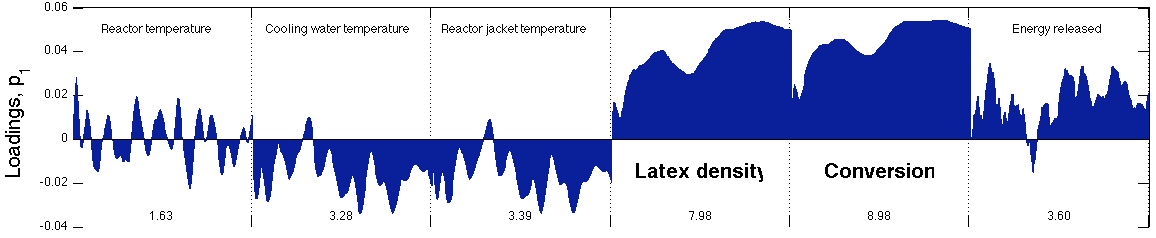
\includegraphics[width=\textwidth]{images/sbr/SBR-loadings-p1.png}
	\end{center}
	\begin{center}
		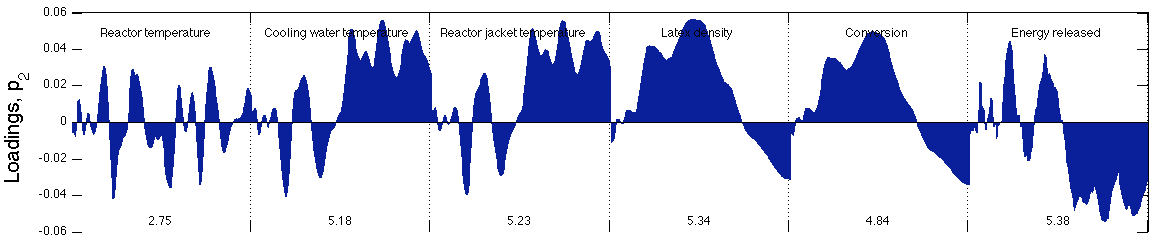
\includegraphics[width=\textwidth]{images/sbr/SBR-loadings-p2.png}
	\end{center}
	
	\begin{itemize}
		\item	Batch 37 [low \( t_1 \)]: below average latex density and conversion throughout the batch
		
		\item	Batch 34:[high \( t_2 \)]: above average cooling water temp, jacket temp, and below avg energy released in last half
		
	\end{itemize}
\end{frame}
 
\begin{frame}\frametitle{SBR: scores \emph{over time} for batch 37}
	
	\begin{center}
		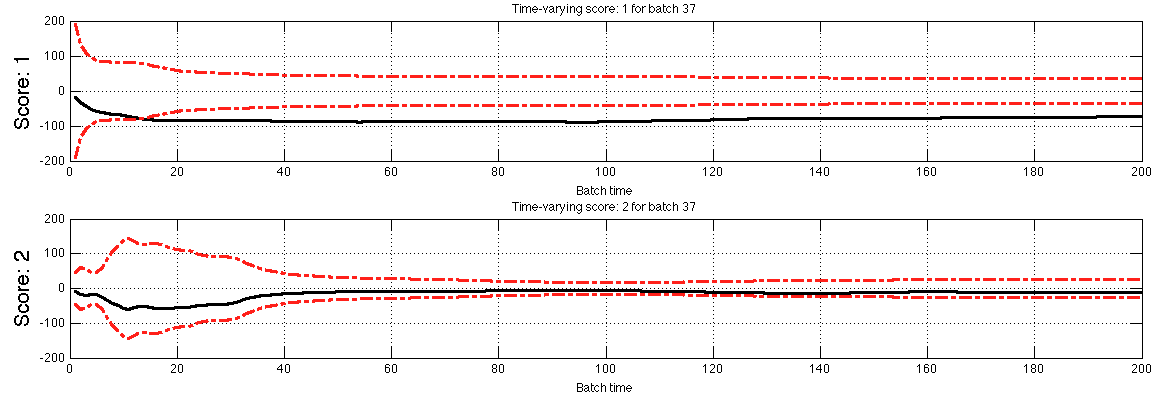
\includegraphics[width=\textwidth]{images/sbr/SBR-time-evolving-scores.png}
	\end{center}
	
	\begin{itemize}
		\item	Don't just have a \( t \)-score at the end, also get the score as batch progresses
		
		\item	Highlights \emph{when} the problem occurred: right at the start
		
				\begin{itemize}
					\item	Was due to an impurity in the feed: consumed reactant and lowers latex density and conversion
				\end{itemize}
	\end{itemize}
	
	{\color{myOrange}{\texttt{plot(batch\_PCA, 'scores', \{'batch', 37\})}}}
\end{frame}

\begin{frame}\frametitle{SBR: contribution plot for batch 37}
	
	\begin{center}
		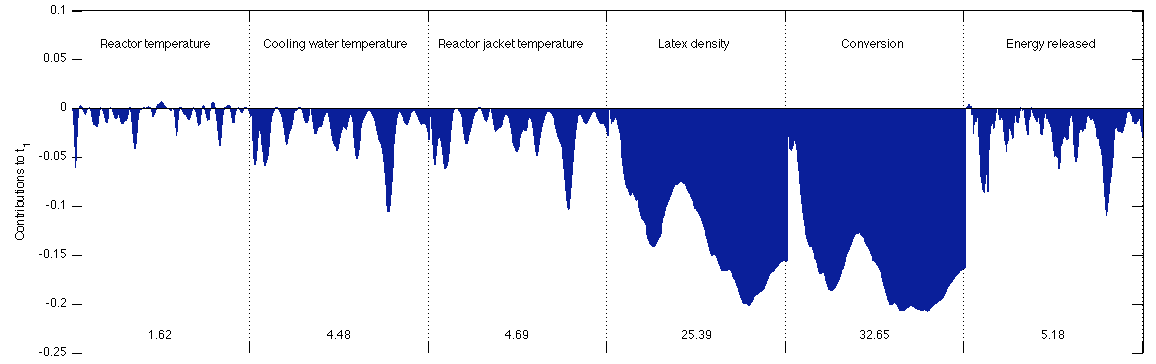
\includegraphics[width=\textwidth]{images/sbr/SBR-contributions-to-batch-37.png}
	\end{center}
	
	\begin{itemize}
		\item	Contributions highest for the latex density and conversion, as expected.
		
				\begin{itemize}
					\item	{\color{myOrange}{\texttt{  contrib\_37 = contrib(batch\_PCA, 37)  }}}
					
					\item	{\color{myOrange}{\texttt{  plot(contrib\_37, 'scores', 1)		  }}}
				\end{itemize}
	\end{itemize}
\end{frame}

\begin{frame}\frametitle{SBR: raw data for batch 37 (to confirm)}
	
	\begin{center}
		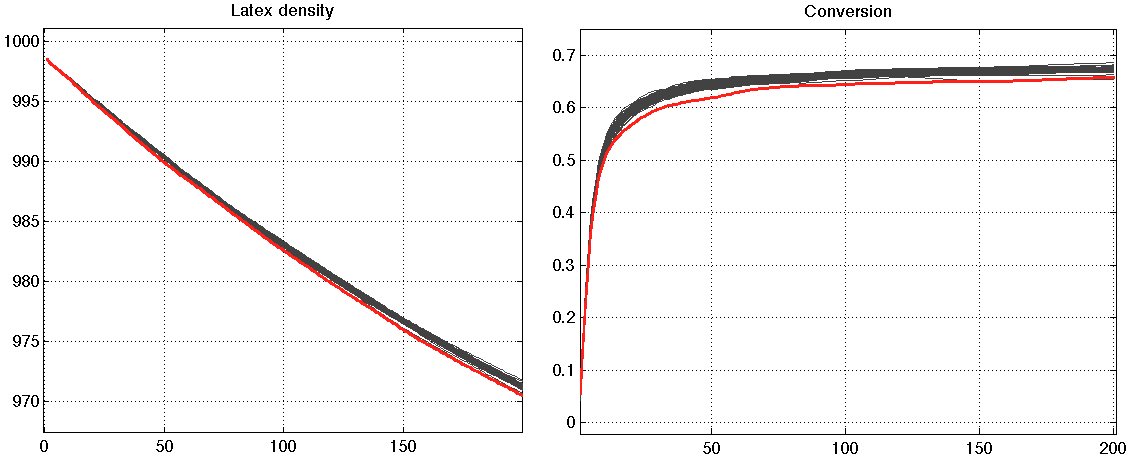
\includegraphics[width=\textwidth]{images/sbr/SBR-raw-data-batch-37-highlighted.png}
	\end{center}
	
	\begin{itemize}
		\item	Confirmed our interpretation with the raw data
				
				\begin{itemize}
					\item	{\color{myOrange}{\texttt{  plot(batch\_PCA.X, 'highlight', 2, 3, 37)		  }}}
					
					\item	uses a \( 2 \times 3 \) layout for the raw tags
				\end{itemize}
	\end{itemize}
\end{frame}

\begin{frame}\frametitle{SBR:  batch 34}
	
	\begin{itemize}		
		\item	Let's investigate this together in the software
		
		\item	Main new learning: SPE trajectories
		
				\begin{itemize}
					\item	SPE values also available during the batch, with limits
					
					\item	{\color{myOrange}{\texttt{  plot(batch_PCA, 'spe', {'batch', 34})		  }}}
					
				\end{itemize}
	\end{itemize}
				
	\begin{center}
		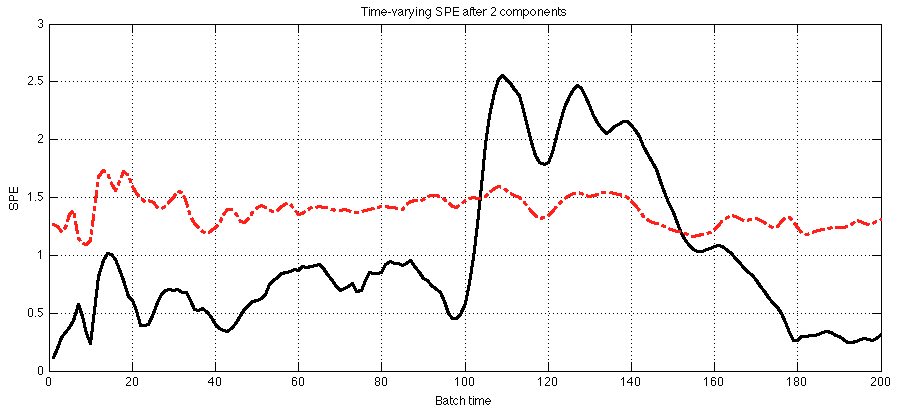
\includegraphics[width=\textwidth]{images/sbr/SBR-time-evolving-SPE-batch-34.png}
	\end{center}
\end{frame}





